Here is a few steps you can take as a guide to training a neural network.\footnote{From Stanford CS 229 NLP.}
\begin{enumerate}
  \item Preprocess the data. 
  \item Choose your neural net architecture (number of layers/neurons, etc.) 
  \item Do a forward pass with the initial parameters, which should be small, and check that the loss is reasonable (e.g. $\log(1/10) \approx 2.3$ for softmax classification of 10 classes). 
  \item Now crank up the regularization term, and your loss should have gone up. 
  \item Now try to train on only a very small portion of your data without regularization using SGD, which you should be able to overfit and get the accuracy to 100\%. 
  \item Now you can train your whole dataset. Start off with a small regularization (e.g. 1e-6) and find a learning rate that makes the loss go down. 
  \begin{enumerate}
      \item Run for a few epochs to see if the cost goes down too slowly (step size is too small) or the cost explodes (step size too big). A general tip is that if the cost is ever bigger than $3$ times the original cost, then this is an indication that the cost has exploded. 
      \item We can run a grid search (in log space) over the learning rate and the regularization hyperparameters over say 10 epochs each, and compare which one makes the most progress. 
  \end{enumerate}
  \item Monitor and visualize the loss curve. 

  \begin{figure}[H]
    \centering 
    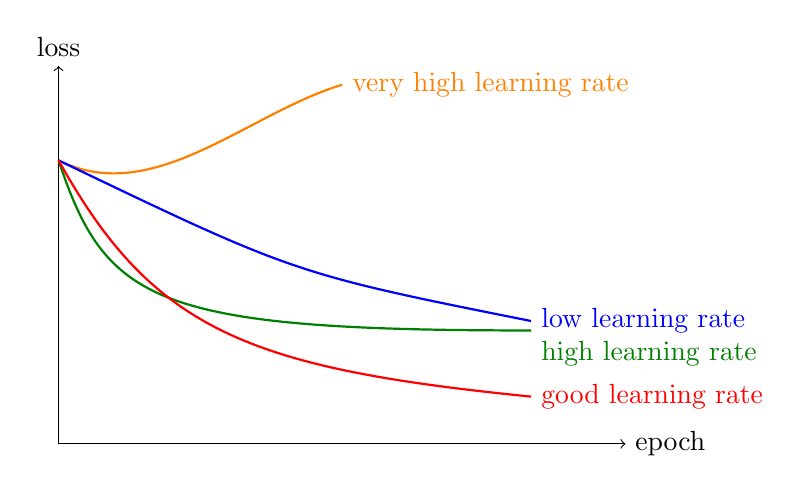
\begin{tikzpicture}[scale=1.2]
      % Set up the axes
      \draw[->] (0,0) -- (6,0) node[right] {epoch};
      \draw[->] (0,0) -- (0,4) node[above] {loss};
      
      % Plot the curves
      % Very high learning rate (yellow)
      \draw[orange, thick] (0,3) .. controls (1,2.5) and (2,3.5) .. (3,3.8) 
          node[right] {very high learning rate};
      
      % Low learning rate (blue)
      \draw[blue, thick] (0,3) .. controls (2.5, 1.8) .. (5,1.3) 
          node[right] {low learning rate};
      
      % High learning rate (green)
      \draw[green!50!black, thick] (0,3) .. controls (0.5,1.5) and (1,1.2) .. (5,1.2)
          node[below right] {high learning rate};
      
      % Good learning rate (red)
      \draw[red, thick] (0,3) .. controls (1,1.2) and (2,0.8) .. (5,0.5)
          node[right] {good learning rate};
    \end{tikzpicture}
    \caption{If you see loss curves that are flat for a while and then start decreasing, then bad initialization is a prime suspect. } 
    \label{fig:loss_curve_diagnostics}
  \end{figure}

  \item We also want to track the ratio of weight updates and weight magnitudes. That is, we can take the norm of the weights $\boldsymbol{\theta}$ and the gradient updates $\nabla \boldsymbol{\theta}$, and a rule of thumb is that the ratio should be about 
  \[\frac{||\nabla \boldsymbol{\theta}||}{||\boldsymbol{\theta}||} \approx 0.001 \text{ or } 0.01\]
\end{enumerate}

